\documentclass[journal,12pt,twocolumn]{IEEEtran}

\usepackage{setspace}
\usepackage{gensymb}
\singlespacing
\usepackage[cmex10]{amsmath}

\usepackage{amsthm}

\usepackage{mathrsfs}
\usepackage{txfonts}
\usepackage{stfloats}
\usepackage{bm}
\usepackage{cite}
\usepackage{cases}
\usepackage{subfig}
\usepackage{graphicx}
\usepackage{longtable}
\usepackage{multirow}

\usepackage{enumitem}
\usepackage{mathtools}
\usepackage{steinmetz}
\usepackage{tikz}
\usepackage{circuitikz}
\usepackage{verbatim}
\usepackage{tfrupee}
\usepackage[breaklinks=true]{hyperref}
\usepackage{graphicx}
\usepackage{tkz-euclide}

\usetikzlibrary{calc,math}
\usepackage{listings}
    \usepackage{color}                                            %%
    \usepackage{array}                                            %%
    \usepackage{longtable}                                        %%
    \usepackage{calc}                                             %%
    \usepackage{multirow}                                         %%
    \usepackage{hhline}                                           %%
    \usepackage{ifthen}                                           %%
    \usepackage{lscape}     
\usepackage{multicol}
\usepackage{chngcntr}

\DeclareMathOperator*{\Res}{Res}

\renewcommand\thesection{\arabic{section}}
\renewcommand\thesubsection{\thesection.\arabic{subsection}}
\renewcommand\thesubsubsection{\thesubsection.\arabic{subsubsection}}

\renewcommand\thesectiondis{\arabic{section}}
\renewcommand\thesubsectiondis{\thesectiondis.\arabic{subsection}}
\renewcommand\thesubsubsectiondis{\thesubsectiondis.\arabic{subsubsection}}


\hyphenation{op-tical net-works semi-conduc-tor}
\def\inputGnumericTable{}                                 %%

\lstset{
%language=C,
frame=single, 
breaklines=true,
columns=fullflexible
}
\begin{document}
\newtheorem{lemma}{Lemma}[section]
\newcommand{\BEQA}{\begin{eqnarray}}
\newcommand{\EEQA}{\end{eqnarray}}
\newcommand{\define}{\stackrel{\triangle}{=}}
\bibliographystyle{IEEEtran}
\raggedbottom
\setlength{\parindent}{0pt}
\providecommand{\mbf}{\mathbf}
\providecommand{\pr}[1]{\ensuremath{\Pr\left(#1\right)}}
\providecommand{\qfunc}[1]{\ensuremath{Q\left(#1\right)}}
\providecommand{\sbrak}[1]{\ensuremath{{}\left[#1\right]}}
\providecommand{\lsbrak}[1]{\ensuremath{{}\left[#1\right.}}
\providecommand{\rsbrak}[1]{\ensuremath{{}\left.#1\right]}}
\providecommand{\brak}[1]{\ensuremath{\left(#1\right)}}
\providecommand{\lbrak}[1]{\ensuremath{\left(#1\right.}}
\providecommand{\rbrak}[1]{\ensuremath{\left.#1\right)}}
\providecommand{\cbrak}[1]{\ensuremath{\left\{#1\right\}}}
\providecommand{\lcbrak}[1]{\ensuremath{\left\{#1\right.}}
\providecommand{\rcbrak}[1]{\ensuremath{\left.#1\right\}}}
\theoremstyle{remark}
\newtheorem{rem}{Remark}
\newcommand{\sgn}{\mathop{\mathrm{sgn}}}
\providecommand{\abs}[1]{\vert#1\vert}
\providecommand{\res}[1]{\Res\displaylimits_{#1}} 
\providecommand{\norm}[1]{\lVert#1\rVert}
\providecommand{\sinc}{sinc}
%\providecommand{\norm}[1]{\lVert#1\rVert}
\providecommand{\mtx}[1]{\mathbf{#1}}
\providecommand{\mean}[1]{E[ #1 ]}
\providecommand{\fourier}{\overset{\mathcal{F}}{ \rightleftharpoons}}
%\providecommand{\hilbert}{\overset{\mathcal{H}}{ \rightleftharpoons}}
\providecommand{\system}{\overset{\mathcal{H}}{ \longleftrightarrow}}
	%\newcommand{\solution}[2]{\textbf{Solution:}{#1}}
\newcommand{\solution}{\noindent \textbf{Solution: }}
\newcommand{\cosec}{\,\text{cosec}\,}
\providecommand{\dec}[2]{\ensuremath{\overset{#1}{\underset{#2}{\gtrless}}}}
\newcommand{\myvec}[1]{\ensuremath{\begin{pmatrix}#1\end{pmatrix}}}
\newcommand{\mydet}[1]{\ensuremath{\begin{vmatrix}#1\end{vmatrix}}}
\numberwithin{equation}{subsection}
\makeatletter
\@addtoreset{figure}{problem}
\makeatother
\let\StandardTheFigure\thefigure
\let\vec\mathbf
\renewcommand{\thefigure}{\theproblem}
\def\putbox#1#2#3{\makebox[0in][l]{\makebox[#1][l]{}\raisebox{\baselineskip}[0in][0in]{\raisebox{#2}[0in][0in]{#3}}}}
     \def\rightbox#1{\makebox[0in][r]{#1}}
     \def\centbox#1{\makebox[0in]{#1}}
     \def\topbox#1{\raisebox{-\baselineskip}[0in][0in]{#1}}
     \def\midbox#1{\raisebox{-0.5\baselineskip}[0in][0in]{#1}}
\vspace{3cm}
\title{EE3900-Gate Assignment}
\author{W Vaishnavi\\AI20BTECH11025}
\maketitle
\newpage
\bigskip
\renewcommand{\thefigure}{\theenumi}
\renewcommand{\thetable}{\theenumi}
Download all latex-tikz codes from 
%
\begin{lstlisting}
https://github.com/vaishnavi-w/EE3900/blob/main/Gate3/latex3.tex
\end{lstlisting}
\section*{Gate EC - 2001 Q1.21}
If a signal $f(t)$ has energy $E$, the energy of the signal $f(2t)$ is equal to 
\begin{enumerate}[label=\Alph*)]
    \item $E$
    \item $\frac{E}{2}$
    \item $2E$
    \item $4E$
\end{enumerate}
\section*{Solution}
The energy of the signal $f(t)$ is given as.
\begin{align}
    E = \int_{-\infty}^{\infty} |f\brak{t}|^2 dt
\end{align}
The energy of signal $f(2t)$,
\begin{align}
    E' = \int_{-\infty}^{\infty} |f\brak{2t}|^2 dt
\end{align}
Putting $u = 2t$,
\begin{align}
    du = 2dt\\
    E' = \int_{-\infty}^{\infty} |f\brak{u}|^2 \frac{du}{2} = \frac{E}{2}
\end{align}
\textbf{Answer}: Option B

\section*{Example}
\begin{lemma}
Parseval's theorem states that there is no loss of information in Fourier transform and the amount of energy remains the same in time and frequency domains.
\begin{align}
    \int_{-\infty}^{\infty} |x\brak{t}|^{2} dt = \int_{-\infty}^{\infty} |X\brak{f}|^{2} df
\end{align}
\end{lemma}
Consider a signal 
\begin{align}
    f\brak{t} = \sinc{\brak{t}}\\
    \sinc{\brak{t}} \fourier rect\brak{f}
\end{align}
where 
\begin{align}
\sinc{\brak{t}} =
    \begin{cases}
    1 & t = 0\\
    \frac{\sin{\pi t}}{\pi t} & otherwise
    \end{cases}\\
    rect\brak{t} =
    \begin{cases}
    1 & \text{if } |t| \leq \frac{1}{2}\\
    0 & \text{if } otherwise
    \end{cases}
\end{align}
Energy of the signal using Parseval's thoerem,
\begin{align}
     \int_{-\infty}^{\infty} \sinc^2{\brak{t}}  dt &= \int_{-\infty}^{\infty} \brak{rect\brak{f}}^2  df \\
     &= \int_{-\frac{1}{2}}^{\frac{1}{2}} df = 1
\end{align}
Consider a signal,
\begin{align}
    f\brak{2t} = \sinc{\brak{2t}}
\end{align}
When a time signal $g\brak{t}$ is time scaled by $\alpha$, the resulting Fourier transform is given by:
\begin{align}
    \label{scale} g\brak{\alpha t} \fourier \frac{1}{\abs{\alpha}}G\brak{\frac{f}{\alpha}}\\
    \implies \sinc{\brak{2t}} \fourier\frac{1}{2}rect\brak{\frac{f}{2}}
\end{align}
Energy of signal,
\begin{align}
    E' &= \int_{-\infty}^{\infty} \sinc^2{\brak{2t}}  dt \\
    &= \int_{-\infty}^{\infty} \brak{\frac{1}{2}rect\brak{\frac{f}{2}}}^2 df \\
    &= \frac{1}{4}\int_{-1}^{1} df = \frac{1}{2} = \frac{E}{2}
\end{align}

\begin{figure}[h]
\centering
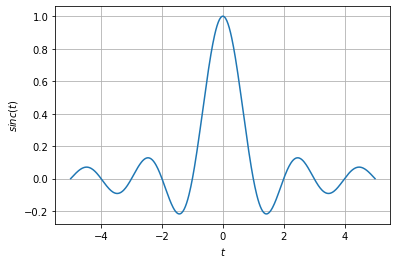
\includegraphics[width=\columnwidth]{sinct.png}
\caption{Plot of signal $f(t)$}
\label{fig:hyperbola}
\end{figure}
\begin{figure}[h]
\centering
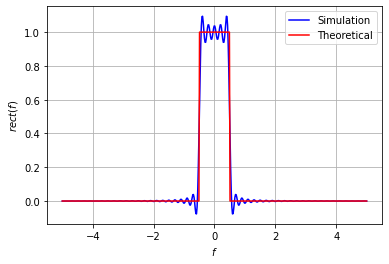
\includegraphics[width=\columnwidth]{fourier_sinc.png}
\caption{Fourier transform of $f(t)$}
\label{fig:hyperbola}
\end{figure}
\begin{figure}[h]
\centering
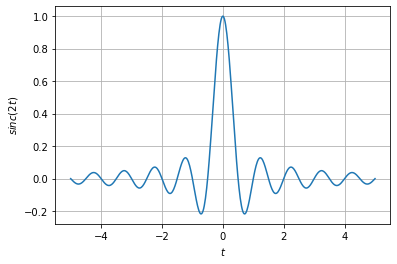
\includegraphics[width=\columnwidth]{sinc2t.png}
\caption{Plot of signal $f(2t)$}
\label{fig:hyperbola}
\end{figure}
\begin{figure}[h]
\centering
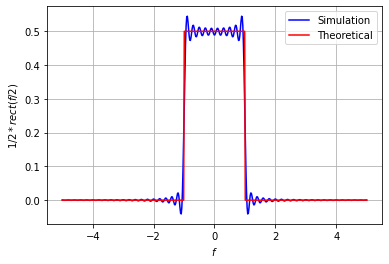
\includegraphics[width=\columnwidth]{fourier_sinc2t.png}
\caption{Fourier transform of $f(2t)$}
\label{fig:hyperbola}
\end{figure}
\end{document}
